\chapter{Resultados} \label{resultados}

\section{Modelos de referência}
O painel solar escolhido para as simulações é um modelo da GOMSpace, o NanoPower P110 \cite{pv_gomspace_datasheet}, a tabela \ref{pv_specs_table} detalha as suas especificações técnicas. Para simular da melhor forma o comportamento do painel nas simulações SPICE, utilizaremos o modelo de aproximação pelos dados do datasheet, conforme apresentado na revisão teórica.

\begin{table}[H]
\centering
\caption{Especificações do NanoPower P110}
\label{pv_specs_table}
\begin{tabular}{|l|l|l|l|l|l|} 
\cline{2-6}
\multicolumn{1}{c|}{} & Condition                  & \multicolumn{1}{c|}{Min} & \multicolumn{1}{c|}{Typ} & \multicolumn{1}{c|}{Max} & Unit  \\ 
\hline
Voltage               & Full Sunlight in LEO       & 4.64                     & -                        & 4.84                     & V     \\ 
\hline
Current               & Current at optimal voltage & 490                      & -                        & 508                      & mA    \\ 
\hline
Power                 & Maximum power              & 2270                     & -                        & 2400                     & mW    \\ 
\hline
Efficiency            &                            & 29.8                     & 30                       & 30.2                     & \%    \\
\hline
Temperature coefficient &                            & 0.21                     & 0.233                       & 0.25                     & \%/ºC    \\
\hline
\end{tabular}
\end{table}

\noindent
\begin{minipage}{\linewidth}
\makebox[\linewidth]{
    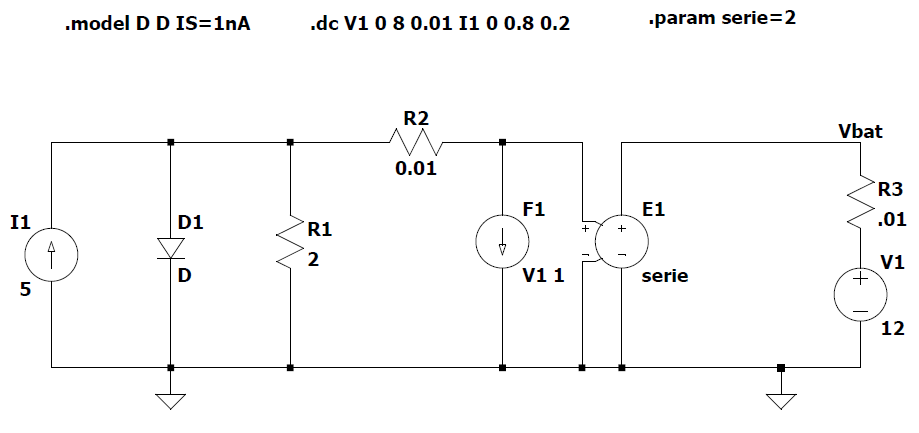
\includegraphics[keepaspectratio=true, scale=0.55]{imagens/PV_model_circuit.png}}
\captionof{figure}{Circuito equivalente para o painel solar}
\label{fig:model_pv_circuit}
\end{minipage}

\noindent
\begin{minipage}{\linewidth}
\makebox[\linewidth]{
    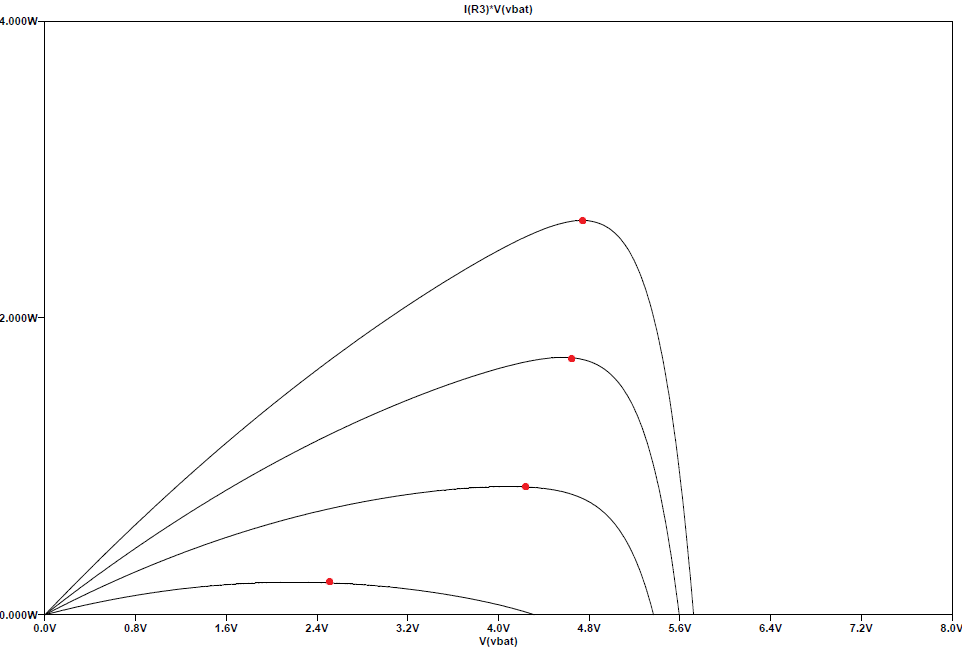
\includegraphics[keepaspectratio=true, scale=0.55]{imagens/PV_model_traces_mpps.png}}
\captionof{figure}{Gráfico de tensão na bateria x potência entregue}
\label{fig:model_pv_traces}
\end{minipage}

No circuito da figura \ref{fig:model_pv_circuit}, além do modelo da célula solar foi colocado um modelo simplificado de bateria consistindo de um fonte de tensão e resistor em série. As fontes lineares dependentes foram adicionadas para simular as células conectadas em série, no caso do painel NanoPower P110 trata-se de duas células 3G30A SCA.

No gráfico \ref{fig:model_pv_traces}, cada uma das curvas dispostas representam irradiações solares distintas, atráves de uma simulação \textit{DC sweep}, alterando as correntes de entrada. A medida que a irradiação solar aumenta, a curva I-V aumenta a sua área e os pontos de máxima potência, marcados em vermelho, se modificam com a tensão de saída no painel solar, o que mostra a necessidade de trabalhar sempre no ponto de máxima potência.  

Para efeitos de simplificação dos esquemáticos, o modelo apresentado estará representado dentro de um modelo customizado no simulador LTSpice chamado de Model\_PV.

Para as baterias, o nosso modelo de referência \cite{battery_gomspace_datasheet} é a bateria Ion-lítio NanoPower 18650 de 2600 mAh. Porém, na questão das baterias, existe uma complexidade a mais, conforme vimos no histórico das missões anteriores, a quantidade e arranjo das células podem variar e isso afeta a condição de carregamento das baterias, por esse motivo, como referência nas simulações, estaremos padronizando a tensão de carregamento na mesma utilizada pelo EPS da GOMSpace, modelo NanoPower P31u \cite{eps_gomspace_datasheet}, que é de 5V.

Para os conversores e controladores, que são os alvos do trabalho, estaremos utilizando os modelos SPICE, fornecidos pelas próprias fabricantes dos chips, sem nenhuma alteração ou customização. 

\subsection*{Cenários de simulação}

Para cada conversor, além do cenário em operação normal, serão apresentados os seguintes cenários:
\begin{itemize}
    \item Transiente da tensão de entrada de 0V até a tensão de operação máxima. Com esse cenário, avalia-se quanto de tensão na entrada é preciso para que o conversor forneça a saída regulada na tensão desejada.
    \item Chaveamento entre desligado e ligado. Nesse cenário, avalia-se a resposta do conversor ao degrau, ou seja, o transiente de quanto o conversor é ligado, o que se traduz em um baixo tempo de resposta, ou seja, o tempo necessário para que a tensão na saída esteja estabilizada é pequeno.
    \item Alterações na carga durante a simulação já com o circuito no estado estável. Uma carga extra será inserida no meio da simulação. Nesse cenário, estamos interessados na resposta do conversor a essa situação. Quanto tempo é necessário para restaurar a operação normal e o quanto de queda de tensão está presente. 
\end{itemize}


\section{Topologia discreta}

\subsection*{LM2735}

\noindent
\begin{minipage}{\linewidth}
\makebox[\linewidth]{
    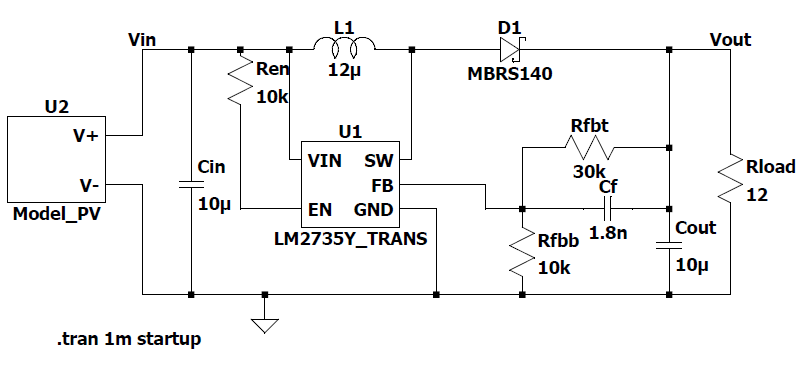
\includegraphics[keepaspectratio=true, scale=0.75]{imagens/LM2735/LM2735_stock_05.png}}
\captionof{figure}{Circuito do LM2735 em condições normais}
\label{fig:lm2735_stock}
\end{minipage}

O LM2735 \cite{lm2735_datasheet} é um conversor DC-DC fabricado pela Texas Instruments, que pode ser usado na configuração Boost ou SEPIC. É um conversor com um \textit{pinout} relativamente pequeno, pois muitas das suas funções são internas e fixas, conforme definido pelo fabricante. Alguns exemplos são o \textit{soft-start} interno e fixo em 4 ms, compensação interna, a frequência de chaveamento fixa em 520 kHz, todas essas funcionalidades internas e fixas poupam a existência de pinos de configuração e ajuda a diminuir o espaço consumido pelo circuito integrado dentro da PCB. O conversor conta ainda com a presença um pino de \textit{Enable} ativo alto. A tabela \ref{lm2735_specs_table} mostra as especificações de operação.

\begin{table}
\centering
\caption{Especificações do LM2735Y}
\label{lm2735_specs_table}
\begin{tabular}{|l|l|l|l|l|} 
\cline{2-5}
\multicolumn{1}{c|}{} & \multicolumn{1}{c|}{Min} & \multicolumn{1}{c|}{Typ} & \multicolumn{1}{c|}{Max} & Unit  \\ 
\hline
Input                 & 2.7                      & -                        & 5.5                      & V     \\ 
\hline
Output                & 3                        & -                        & 24                       & V   \\ 
\hline
Switch current                & -                        & -                        & 2.1                      & A   \\ 
\hline
Switching Frequency   & 360                        & 520                      & 580                        & kHz   \\
\hline
Duty Cycle   & 2                        & 99 ($T_{J}$ = 25ºC)                      & 91                        & \%   \\
\hline
\end{tabular}
\end{table}

\noindent
\begin{minipage}{\linewidth}
\makebox[\linewidth]{
    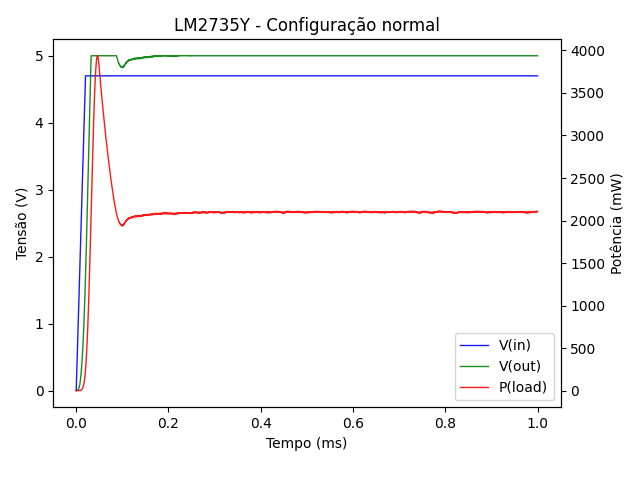
\includegraphics[keepaspectratio=true, scale=1]{imagens/LM2735/5V@05A.png}}
\captionof{figure}{Resposta do LM2735 em condições normais}
\label{fig:lm2735_traces_stock}
\end{minipage}

Um ponto fundamental do regulador chaveado frente ao regulador linear é a eficiência energética. Um regulador chaveado consegue chegar a eficiência de potência da ordem de 90\%. A eficiência é importantíssima no cubesat, que está em um ambiente com fonte limitada de energia, fonte essa que também é intermitente: depende se o satélite está em eclipse ou não.

Analisando a resposta da figura \ref{fig:lm2735_traces_stock}, essa configuração \ref{fig:lm2735_stock} atingiu uma eficiência de 87.8\%, com aproximadamente 2.115 W sendo entregues para a carga.
A tensão $V_{pp}$ de ripple na saída ficou em 12.64 mV, dentro da faixa de valores esperada. Vale ressaltar que esse resultado considera a frequência fixa de chaveamento do conversor de 520 kHz, porém a Texas em seu datasheet explicita que esse valor é válido para $T_{J}$ = 25 ºC, para a faixa de temperaturas de operação que é $T_{J}$ entre -40 ºC e 125 ºC, essa frequência pode oscilar entre 360 e 680 kHz. Portanto, o fato do modelo SPICE não simular os efeitos da temperatura no circuito coloca essa limitação.

\noindent
\begin{minipage}{\linewidth}
\makebox[\linewidth]{
    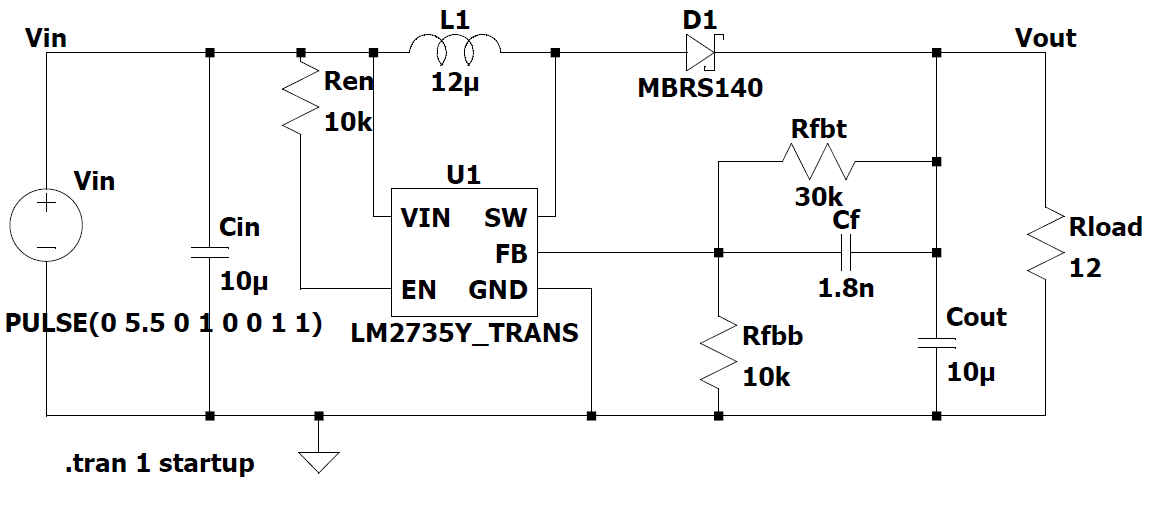
\includegraphics[keepaspectratio=true, scale=0.55]{imagens/LM2735/LM2735_transient_05.png}}
\captionof{figure}{Circuito do LM2735 em transiente de tensão}
\label{fig:lm2735_transient}
\end{minipage}

\noindent
\begin{minipage}{\linewidth}
\makebox[\linewidth]{
    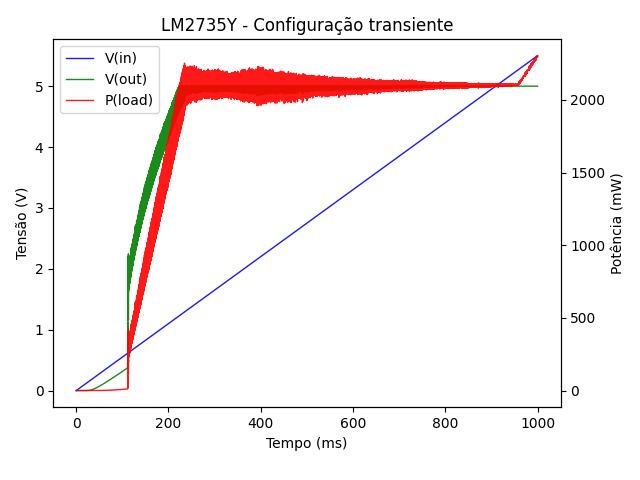
\includegraphics[keepaspectratio=true, scale=1]{imagens/LM2735/5V@05A_transient.png}}
\captionof{figure}{Resposta do LM2735 em transiente de tensão}
\label{fig:lm2735_traces_transient}
\end{minipage}

A figura \ref{fig:lm2735_traces_transient} mostra a resposta quando temos o transiente de tensão aplicado, para isso substituimos o painel solar por uma fonte de tensão do tipo PULSE, que foi programada para executar uma rampa de 0 até 7 V em 1 s. Observa-se que quando a tensão de entrada ultrapassa o valor de aproximadamente 1.3V já é possível observar uma tensão na saída, porém com uma tensão de \textit{ripple} bastante elevada de 330.14 mV, fora da tolerância. Quando a tensão mínima de entrada do conversor (2.7 V) é atingida, é possível obter uma tensão de saída próxima do alvo de 5 V e com a tensão de \textit{ripple} dentro da tolerância de 5\% do valor da saída, com 115.14 mV. Esse ripple vai diminuindo a medida que a tensão na entrada aumenta para a tensão esperada do ponto de máxima potência do painel solar e a para as tensões de entrada superiores as esperadas para o painel, a saída se satura em aproximadamente 5.1 V.

\noindent
\begin{minipage}{\linewidth}
\makebox[\linewidth]{
    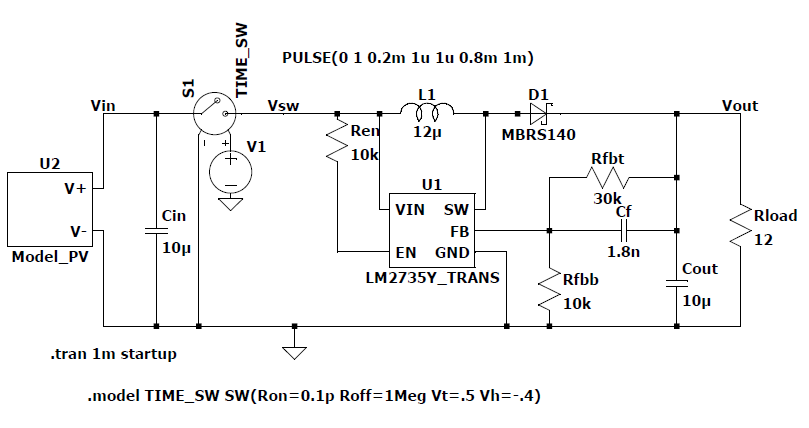
\includegraphics[keepaspectratio=true, scale=0.75]{imagens/LM2735/LM2735_switch_05.png}}
\captionof{figure}{Circuito do LM2735 com chaveamento}
\label{fig:lm2735_switch}
\end{minipage}

\noindent
\begin{minipage}{\linewidth}
\makebox[\linewidth]{
    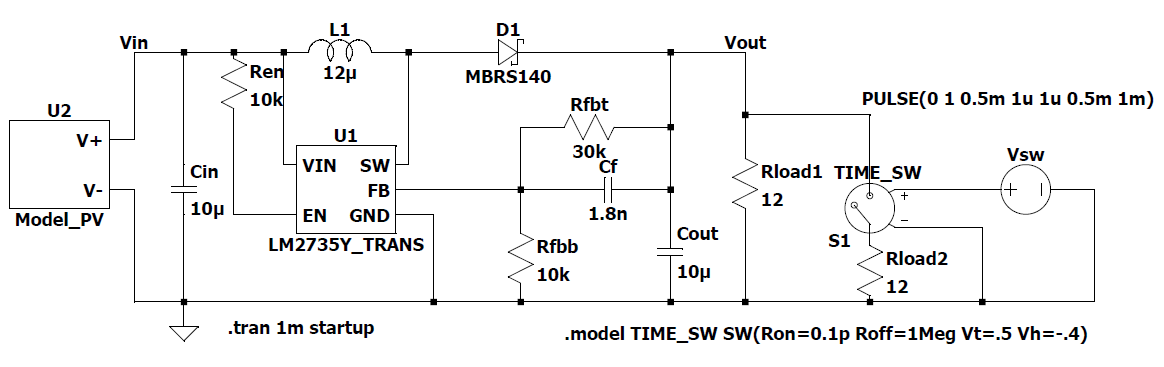
\includegraphics[keepaspectratio=true, scale=0.55]{imagens/LM2735/LM2735_current_05.png}}
\captionof{figure}{Circuito do LM2735 com alteração na carga}
\label{fig:lm2735_current}
\end{minipage}

\noindent
\begin{minipage}{\linewidth}
\makebox[\linewidth]{
    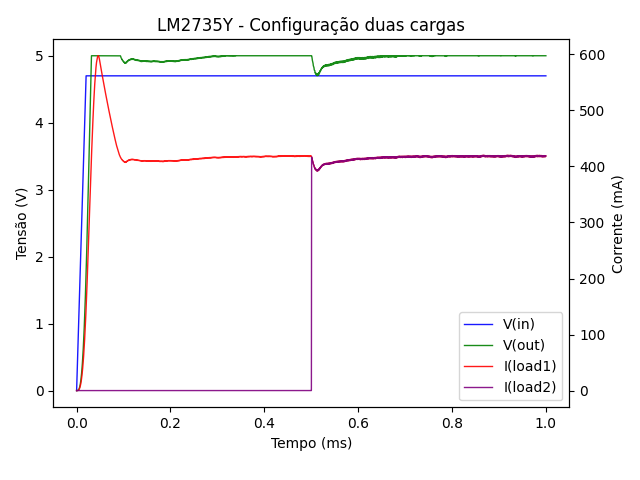
\includegraphics[keepaspectratio=true, scale=1]{imagens/LM2735/5V@05A_current.png}}
\captionof{figure}{Resposta do LM2735 com alteração na carga}
\label{fig:lm2735_traces_current}
\end{minipage}

As figuras \ref{fig:lm2735_current} e \ref{fig:lm2735_traces_current} mostram a resposta do conversor quando uma segunda carga resistiva de 5 $\Omega$ é inserida no circuito, a chave foi programada para ligar em t=0.5 ms, observa-se que o conversor consegue retomar a situação estável em 0.155 ms após o chaveamento da segunda carga, com uma queda de tensão na saída de 0.32V. O tempo de resposta foi bastante parecido com o chaveamento entre ligado e desligado (única carga de 12 $\Omega$) que foi de 0.191 ms, conforme figura \ref{fig:lm2735_traces_switch}, porém a tensão de \textit{ripple} na saída é afetada, passando de 10.05 mV para 28.31 mV, mais do que o dobro da tensão com apenas uma carga.

\noindent
\begin{minipage}{\linewidth}
\makebox[\linewidth]{
    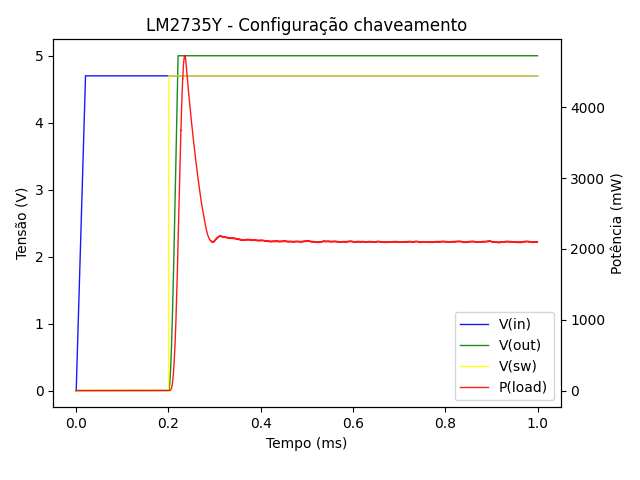
\includegraphics[keepaspectratio=true, scale=1]{imagens/LM2735/5V@05A_switch.png}}
\captionof{figure}{Resposta do LM2735 com chaveamento}
\label{fig:lm2735_traces_switch}
\end{minipage}

\section{Controlador Integrado}

\subsection*{SPV1040}

Para a solução integrada, utilizaremos de referência o SPV1040 \cite{spv1040_datasheet} da ST Microelectronics, o mesmo utilizado na missão ESTCube-1. 

Conforme explicado no capítulo \ref{desenvolvimento}, o SPV1040 é um controlador completo, dessa forma, o \textit{Duty Cycle} é internamente controlado pelo algoritmo de MPPT, o que no caso desse componente é o algoritmo Pertuba e Observa. A tensão de entrada $V_{in}$ opera entre os valores de 0.3 e 5.5 V, o é que suficiente para o painel solar escolhido e a frequência de chaveamento é fixa em 100 kHz. Além de já fornecer a saída regulada, possui também proteção contra superaquecimento e sobrecorrente. Dependendo da configuração, o datasheet mostra que a eficiência dele pode chegar em até 95\%, sendo extremamente indicado para essas situação onde é preciso lidar com tensões de entrada baixas. 

O dispositivo fornece saída regulada de tensão e corrente detectando a tensão $V_{CTRL}$ de \textit{feedback} do divisor de resistor externo, que define a tensão na bateria, e pela queda de tensão no resistor de detecção externa $R_{S}$, respectivamente.

Existem 5 modos de operação possíveis para o controlador:
\begin{enumerate}
    \item Start-up: Quando a tensão de saída $V_{out}$ está acima 0.8 e abaixo 2 V, o dispositivo entra no modo start-up, pois nessa condição a polarização dos MOSFET's de compensação (\textit{BIAS}) ainda não é garantida. Em tais condições, o transistor canal N é forçado a ligar com um duty cycle fixo.
    \item MPPT: Uma vez que o dispositivo saiu do modo start-up, o dispositivo entra no modo MPPT, que utiliza o algoritmo Perturba e Observa.
    \item Shutdown: Modo com o menor consumo energético possível, ativado quando o pino XSHUT está em LOW.
    \item Burst: O modo burst é a transição para o modo sleep-in, o conversor DC-DC começa a operar em frequências cada vez mais lentas. O modo burst atua quando a tensão de saída atinge a tensão da bateria, o pino MPP-SET abaixa de 0.45V ou a corrente de saída atinge o seu valor máximo.
    \item Sleep-in: Nesse modo, nenhuma corrente é fornecida para a carga e esse estado permanece até que a condição que colocou o dispositivo em Sleep-in não esteja mais presente.
\end{enumerate}

A figura \ref{fig:spv1040_block} mostra o diagrama de blocos do dispositivo e a figura \ref{fig:spv1040_sample} mostra o esquemático do circuito necessário para uma saída de 3.8 V com 500 mA, o equivalente para uma bateria de referência da GOMSpace.

\noindent
\begin{minipage}{\linewidth}
\makebox[\linewidth]{
    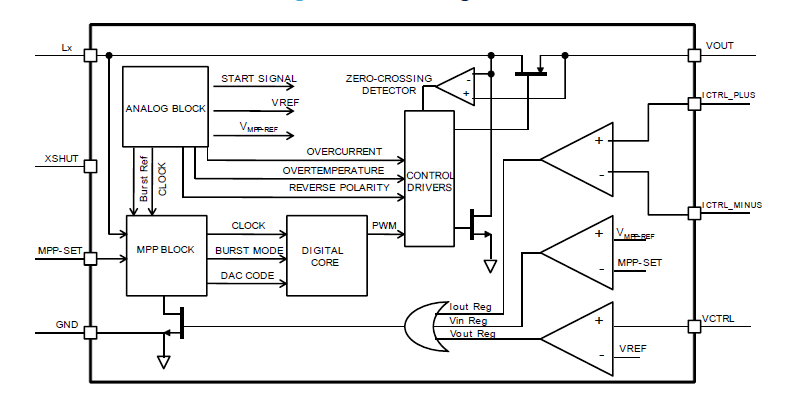
\includegraphics[keepaspectratio=true, scale=0.8]{imagens/SPV1040/SPV1040_block.png}}
\captionof{figure}{SPV1040: Diagrama de blocos}
\label{fig:spv1040_block}
\end{minipage}

\noindent
\begin{minipage}{\linewidth}
\makebox[\linewidth]{
    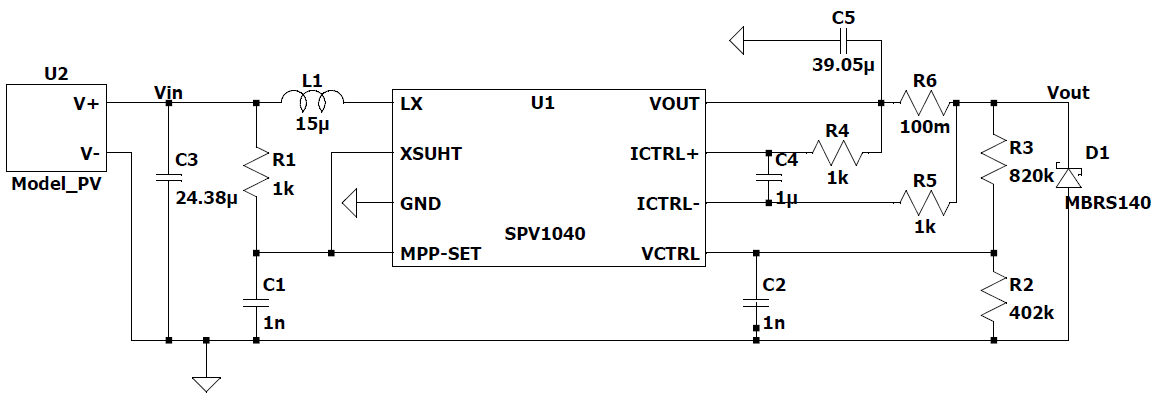
\includegraphics[keepaspectratio=true, scale=0.75]{imagens/SPV1040/SPV1040_sample.png}}
\captionof{figure}{SPV1040 configurado para 3.8 V @ 500 mA}
\label{fig:spv1040_sample}
\end{minipage}